In order to reduce the overlap with other analyses, especially those containing
multijet final states, an upper cut on the number of \gls{hs} jets is
necessary. This procedure is denominated \emph{jet veto}. In order to define
hard scatter jets, cuts on the jet $\pt$ and on the JVT (see
\cref{sec:jet-vertex-tagger}) have been studied. The aim of these cuts is to
render the analysis independent from pile-up as much as possible but stay
signal efficient, too hard cuts would lead to disregarding possible signal
events while, on the other hand, too loose cuts let pile-up jets in the signal
region.

Due to the jets coming from the squark decays, the SUSY compressed
squark-neutralino model have more jets compared to other signals considered in
the monojet analysis and are therefore the most sensitive to jet veto efficiency
and to the definition of hard scatter jet. To study the pile-up contamination
of different $\pt$ thresholds a \emph{figure of merit} is defined and its
dependence from the average number of proton-proton collisions per bunch
crossing studied. The figure of merit is defined as:
\begin{equation}
  \label{eq:fig_merit}
  \frac{\text{N (events) with baseline cuts + at
      most N (jet) HS jets}}{\text{N (events)
      with baseline cuts}}
\end{equation}
where the baseline cuts are the event selection given in
\cref{sec:event-selection} except the cut F (the study presented here uses
$\met = \pt = 250$ GeV) and the hard scatter jets are defined as:
\begin{itemize}
\item Jets with $\pt > 50$ GeV or $|\eta| > 2.4$ (forward jets), are always
  considered coming from the hard scatter.
\item In order to be considered coming from the hard scatter proton-proton
  collision, the jets with $p_T^{\text{thresh}} \leq \pt \leq 50$ GeV must
  additionally satisfy a JVT $>$ JVT$^{\text{ thresh}}$ selection criteria where
  different $p_T^{\text{thresh}}$ and JVT$^{\text{ thresh}}$ have been studied,
  in particular
  $p_T^{\text{thresh}} \in \{30~\text{GeV}, 40~\text{GeV}, 50~\text{GeV},
  70~\text{GeV}\}$ and JVT$^{\text{ thresh}} \in \{0.14, 0.64, 0.92\}$.
\end{itemize}

\cref{fig:comp_4jets_nojvt} shows the jet veto efficiency for the different
values of $p_T^{\mathrm{\, thresh}}$ and N~(jets)~$\leq~4$ in the case where no
JVT cut is applied. In the case of $p_T^{\mathrm{\, thresh}}$ of 30 GeV the
pile-up dependence is noticeable while it becomes less important with tighter
cuts. In \cref{fig:comp_4jets_jvt64} a JVT $>$ 0.64 selection is applied in the
definition of the hard scatter jets, in this case the pile-up dependence for
the $p_T^{\mathrm{\, thresh}}$ of 30 GeV is reduced and the distribution for
$p_T^{\mathrm{\, thresh}}$ of 40, 50 and 70 GeV cuts is, within statistical
error, flat.
\begin{figure}[!h]
  \centering
  \begin{subfigure}[t]{.48\linewidth}
    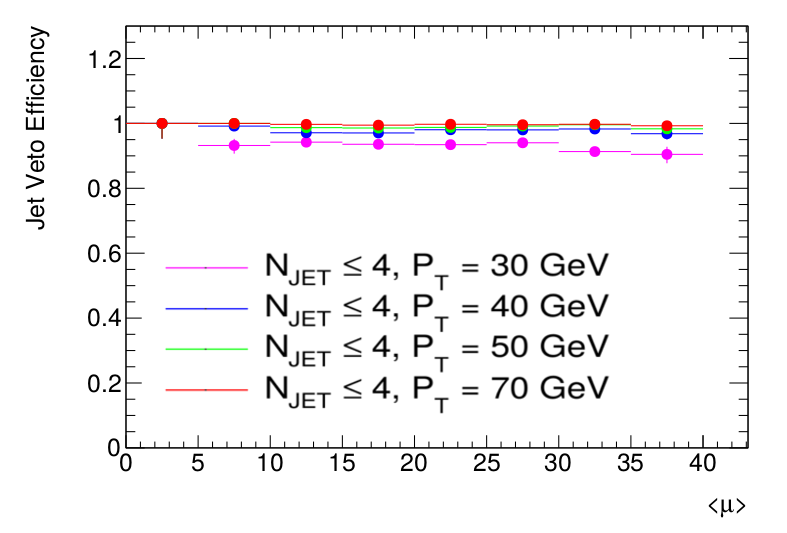
\includegraphics[width=\linewidth]{Compressed_450_435_mu_4jets_M0}
    \caption{No JVT cut applied.}
    \label{fig:comp_4jets_nojvt}
  \end{subfigure}
  \begin{subfigure}[t]{.48\linewidth}
    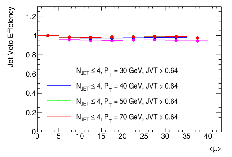
\includegraphics[width=\linewidth]{Compressed_450_435_mu_4jets_jvt64_M0}
    \caption{JVT > 0.64.}
    \label{fig:comp_4jets_jvt64}
  \end{subfigure}
  \caption{Jet veto efficiency for different jet $\pt$ thresholds and N (jets)
    $\leq 4$ as a function of the average number of interactions per bunch
    crossing $<\mu>$ for a compressed spectra model point $\msquark = 450$ GeV
    $\mneutralino = 435$ GeV. In Figure~\ref{fig:comp_4jets_nojvt} no JVT cut is
    applied and there is some drop of the efficiency at high pile-up. In
    Figure~\ref{fig:comp_4jets_jvt64} a JVT $> 0.64$ cut is applied, the
    dependence from pile-up is reduced.}
  \label{fig:comp_eff}
\end{figure}
The effect of the upper cuts on the number of hard scatter jets with the default
definition used in this analysis on the signal models considered is
verified. \cref{fig:jet_veto_comparison} shows the same behavior described above
on the $\znunu$ background. Also in this case an improvement of the jet veto
efficiency as function of the average number of interaction per crossing
especially for $\pt = 30$~GeV is seen. The selected definition of the
hard-scatter jets, with N (jets) $\leq$ 4 is, within statistical error, 99\%
efficient for the considered signals.
\begin{figure}[!h]
  \centering
  \begin{subfigure}[t]{.48\linewidth}
    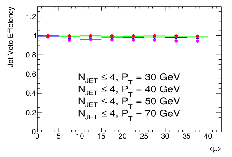
\includegraphics[width=\linewidth]{Znunu_mu_4jets_M0}
    \caption{No JVT cut applied.}
    \label{fig:znunu_4jets_jvt64}
  \end{subfigure}
  \begin{subfigure}[t]{.48\linewidth}
    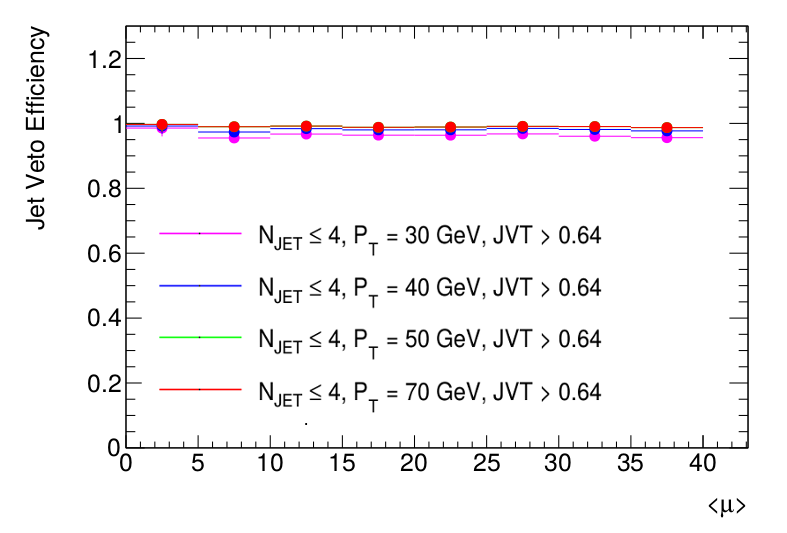
\includegraphics[width=\linewidth]{Znunu_mu_4jets_jvt64_M0}
    \caption{JVT > 0.64.}
    \label{fig:comp_4jets_jvt64_1}
  \end{subfigure}
  \caption{Jet veto efficiency for different jet $\pt$ thresholds and N (jets)
    $\leq 4$ as a function of the average number of interactions per bunch
    crossing $<\mu>$ for the $\znunu$ background. In
    Figure~\ref{fig:comp_4jets_nojvt} no JVT cut is applied and there is some
    drop of the efficiency at high pile-up. In Figure~\ref{fig:comp_4jets_jvt64}
    a JVT $> 0.64$ cut is applied, the dependence from pile-up is reduced.}
  \label{fig:jet_veto_comparison}
\end{figure}
%%% Local Variables:
%%% mode: latex
%%% TeX-master: "../search_for_DM_LED_with_ATLAS"
%%% End:
